%% 4. 「技術研究報告」
\documentclass[technicalreport]{ieicej}
%\usepackage[dvips]{graphicx}
\usepackage[dvipdfmx]{graphicx,xcolor}
\usepackage[T1]{fontenc}
\usepackage{lmodern}
\usepackage{textcomp}
\usepackage{latexsym}
%\usepackage[fleqn]{amsmath}
\usepackage{amssymb}
\usepackage{subfigure}

\jtitle{ LTE 環境における応答遅延特性の時系列モデリングによる分析}
\jsubtitle{}
\etitle{Analysis of delay characteristics of connection through LTE by time series analysis}
\esubtitle{}
\authorlist{%
 \authorentry[k-yamamt@ist.osaka-u.ac.jp]{山本 航平}{Kohei YAMAMOTO}{Osaka}
 \authorentry[wakamiya@ist.osaka-u.ac.jp]{若宮 直紀}{Naoki WAKAMIYA}{Osaka}
 \authorentry[ryo.nakano.xd@hitachi.com]{中野 亮}{Ryo NAKANO}{hitachi}
 \authorentry[ryosuke.fujiwara.mb@hitachi.com]{藤原 亮介}{Ryosuke FUJIWARA}{hitachi}
% \authorentry[メールアドレス]{和文著者名}{英文著者名}{所属ラベル}
}
\affiliate[Osaka]{大阪大学大学院情報科学研究科バイオ情報工学講座\\ 〒565-0871 大阪府吹田市山田丘 1-5}{Department of Bioinformatic engineering,Graduate school of Information Science and Technology,Osaka University\\ 1-5 Yamadaoka, suita-shi, Osaka, 565-0871, Japan}
\affiliate[hitachi]{株式会社日立製作所 研究開発グループ\\ 〒185-8601 東京都国分寺市東恋ヶ窪 1-280}{Research \& Development Group, Hitachi, Ltd.\\ 1-280 Higashikoigakubo, kokubunji-shi, Tokyo, 185-8601, Japan}
%\affiliate[所属ラベル]{和文勤務先\\ 連絡先住所}{英文勤務先\\ 英文連絡先住所}

\begin{document}

\newcommand{\argmin}{\mathop{\rm arg~min}\limits}
\def \vector#1{\mbox{\boldmath $#1$}}

\begin{jabstract}
%和文あらまし
産業用モニタリングシステムにおける運用管理コストの低減のため,迅速な障害検知・予測,ならびに原因の特定と対処法の提示が求められている.その実現にむけて,無線機器からサーバまでのLTE回線を含む通信路について,異なる時間帯において応答遅延の計測を行った.本稿では,遅延の変動特性や,曜日や時間帯に依存した傾向の有無について,時系列モデルを用いたクラスタリングによって分析した結果を示す.
\end{jabstract}
\begin{jkeyword}
%和文キーワード
Long Term Evolution,応答遅延,時系列モデリング,異常検知
\end{jkeyword}
\begin{eabstract}
%英文アブストラクト
In order to reduce the costs of operation and management in industrial monitoring systems, it is necessary to detect or predict failures quickly, identify the cause, and present countermeasures. To achieve this, we measured response delays of connection from one wireless device to one server, includeing LTE, in different time zones.In this technical report, we show the results of analyzing the fluctuation characteristics of responce delay and the tendency depending on the day of week or time zone by clustering using a time series analysis.
\end{eabstract}
\begin{ekeyword}
%英文キーワード
Long Term Evolution,response delay,time series analysis,anomaly detection
\end{ekeyword}
\maketitle

\section{はじめに}
近年,IoT (Internet of Things) 技術の発展とともに産業用モニタリングシステム\cite{monitering}が普及している.
これは,工場などの産業施設に設置された機器から直接,あるいは配置したカメラやセンサーなどの IoT デバイスを通じて,機器の稼働状態に関する情報をリアルタイムで収集し,キャリア回線を通じてクラウドサーバに送信,さらにクラウドサーバでデータ処理を行い,運用管理担当者に提示するものである.
従来作業員が巡回し行っていた工場内の機器の点検業務を自動化できるため,人員コストの軽減,目視確認より生じる人的ミスの低減,リアルタイムなデータの利活用などの効果が期待できる.
一方で,長期間の運用のなかで機器に具備された IoT デバイスの故障,工場内ネットワークの通信の途絶,クラウドサーバへの通信の遅延などの障害は避けられない.
このような障害が発生した場合には工場内の機器の稼働状況を把握することが困難となり,工場の稼働停止や業務の遅れなどが引き起こされ大きな損失をもたらす可能性がある.

障害発生時には迅速な復旧作業が求められるが,障害はその原因や内容,規模よってさまざまである.
しかしながら,現状ではシステムから得られる情報を用いてこれらの障害を適切かつ迅速に区別することが困難であるため,障害発生時には運用管理担当者が直接現場に行き障害の原因や内容,規模を確認する必要があり,多大な運用管理コストが発生している.
そのため,モニタリングシステムによる運用管理コストの低減のためには,直接また間接的に取得できる情報にもとづいて,障害発生を迅速に検知また予測するとともに,障害の原因を特定し,加えてその対処法を示すことが求められている.

すでに我々の研究グループでは機器間で測定される受信電波強度の時間変化にもとづいて空間的な電波伝搬特性の変動を推定することにより工場内での無線通信の異常を検知する手法を提案している\cite{prev}.
そこで,本報告では工場内で機器稼働情報を収集する無線機器からクラウドサーバまでの通信路で発生する異常の検知にむけてさまざまな曜日,時間帯で応答遅延を計測し特性の分析を行う.
具体的には,キャリア回線として産業用モニタリングシステムに広く用いられている LTE(Long Term Evolution)回線を用いる.
LTE 回線に関する研究として,応答遅延時間を他の無線回線と比べて評価を行った研究\cite{lte1}\cite{lte2}や LTE 環境下での TCP パケットの振る舞いに関する調査\cite{tcp},LTE 環境の応答遅延において,人の混雑状況にかかわらず発生する低遅延帯の分布が部分正規分布に従うことを示唆した研究\cite{distribution}などが行われている.
しかし,LTE を利用したインターネットとの通信において発生する遅延などの異常を検知・予測するといった観点からの通信特性の多角的な分析は十分になされていない.
そこでまずは分析に用いる実測データの収集として,月曜日から日曜日の 3 時,7 時,12 時,17 時,20 時のそれぞれ 1 時間において私が在籍している研究室内に設置した無線端末から AWS サーバへ ping による応答遅延の計測を行った.
計測した応答遅延に,例えば曜日,時間帯に依存した傾向が認められれば,その傾向と対比することによって応答遅延の通常ではない振る舞い,すなわち異常を検知することができる.
そこで,時系列モデリングによる回帰で得られたパラメータやその主成分を用いてクラスタリングすることで計測データをグループ化し,共通する特徴を見いだす.

第 2 章では本報告で実施した計測実験の設定について述べる.
第 3 章では時系列モデルによる回帰について述べる.
第 4 章では回帰結果に用いたクラスタリングにもとづく分析について述べる.
第 5 章では全体のまとめと今後の課題について述べる.
\section{計測実験の設定}
本報告では図 \ref{exp} に示す構成で計測実験を行った.
モニタリングシステムにおける無線端末としては LTE モジュールとして Quectel 社製 EC21-J を搭載した Raspberry Pi を用いた.
また,LTE 回線としては IIJ モバイル社のサービスタイプ D 定額プランライト(いちねん プリペイド)を用いた.
IIJ モバイル社は他の通信事業者から通信回線を借り受け,サービスを提供している MVNO(Mobile Virtual Network Operator)であり,サービスタイプ D では NTT ドコモ社の回線を使用している.
月あたり通信量が 3GB を超過すると通信速度が 256kbps に制限されるが,本実験中には速度制限は課されなかった.

クラウドサーバとしては本計測を行うにあたり契約した一台の AWS サーバを用い,大阪大学敷地内の研究室に設置した Raspberry Pi から ping を用いて応答遅延を計測した.
自動的に計測データを取得できるよう,Raspberry Pi 上で動作する Raspbian において計測用のスクリプトを用いることで, 15 秒毎に時刻を取得し,続けて ping (パケットサイズ 60 バイト, ICMP ECHO メッセージ,パケット数 1 )を実行した.
計測時刻,ping の出力をログデータとして取り出し,分析を行った.
また,日時が応答遅延に与える影響を調べるため,様々な時間帯で計測を行った.
計測は 2/29(土)から 3/27(金)までの四週間に渡って行った.

\begin{figure}[tb]
\centering
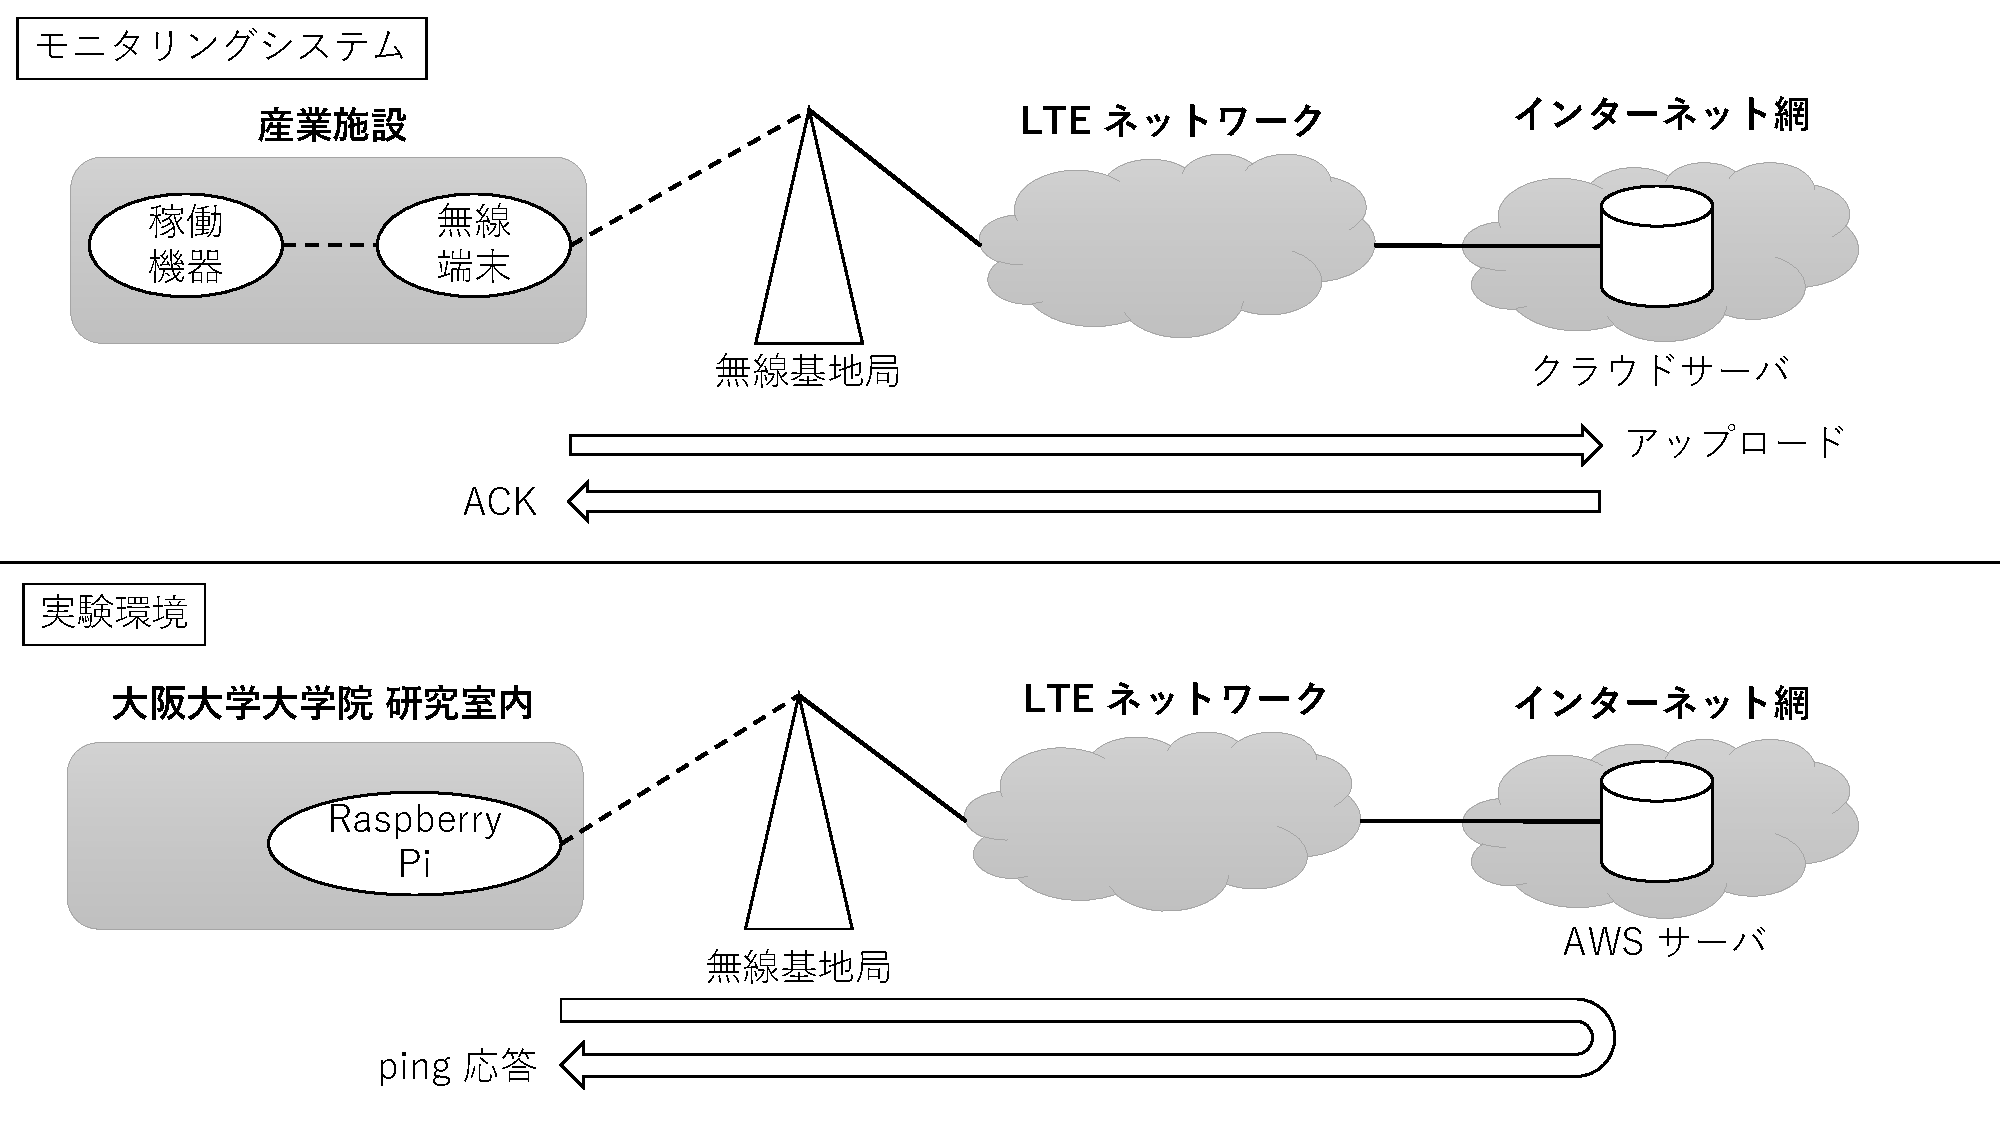
\includegraphics[width=7.5cm]{experiment.pdf}
\caption{モニタリングシステムと実験環境の対応図}
\label{exp}
\end{figure}

\section{時系列モデルによる回帰}
本報告では,時系列モデルとして式 (\ref{garch1}) と式 (\ref{garch2}) で表される ARMA-GARCH(Autoregressive Moving Average - Generalized Autoregressive Conditional Heteroscedasticity)モデル\cite{arma-garch}を用いる.
\begin{equation}
y_t = \sum_{i=1}^p a_i y_{t-i} + \sum_{i=1}^q b_i \varepsilon_{t-i} + c + \varepsilon_{t} 
\label{garch1}
\end{equation}
$$\varepsilon_t \sim N(0,h_t) \hspace{0.5cm} \rm{i.i.d}$$
\begin{equation}
\displaystyle h_{t} = \omega + \sum_{i=1}^{r}\alpha_i\varepsilon_{t-i}^2 + \sum_{i=1}^{s}\beta_ih_{t-i}
\label{garch2}
\end{equation}

時系列モデルによる回帰では,適切な次数 $p,q,r,s$ のもとで実測値 $y_t$ の時系列を最も精度良くモデル化できるパラメータ $a_i,b_i,c,\omega,\alpha_i,$および $\beta_i$ を算出する.
ここで,$y_t(1\leq t\leq N,N=240)$は1時間の計測実験のそれぞれにおける計測時刻順の実測値である.
また,$c$ は定数項,$\varepsilon_t$ は平均0,分散 $h_t$ の独立同一な正規分布に従うノイズ項である.
したがって,時刻 $t$ における実測値 $y_t$ は,過去の $p$ 時点前までの実測値と $q$ 時点前までのノイズ項のそれぞれの重み付き和と自身のノイズ項によって表される.
また,式 (\ref{garch2}) において,$\omega$ は定数項であり,時刻 $t$ におけるノイズ項が従う正規分布の分散 $h_t$ は,過去の $r$ 時点前までのノイズ項と $s$ 時点前までのノイズ項が従う正規分布の分散のそれぞれの重み付き和によって表される.

次数と呼ばれるパラメータ $(p,q,r,s)$ は対象とする時系列データに応じて適切に定める必要がある.
最適な次数は計測実験ごとに異なるが,クラスタリングによる分類,分析のために共通の次数を用いることとする.
次数 $0\leq p\leq2,0\leq q\leq 2,r=1$,および $0\leq s\leq 1$ のそれぞれの組み合わせに対してAIC(赤池情報量規準)\cite{aic1}\cite{aic2}を求めたところ,最大次数である $(p,q,r,s)=(2,2,1,1)$ が最適な計測区間が存在することから,これを共通の次数として用いることとした.
本報告では,式 (\ref{garch1}) に関与する次数 $p,q$ の探索範囲の上限は回帰モデルが複雑になりすぎないようにともに 2 までとし,式 (\ref{garch2}) に関与する次数 $r,s$ の探索範囲の上限は一般的に十分な性能が発揮される 1 まで\cite{hansen2005forecast}とした.
ただ,$r = 0$ は回帰分析を行うにあたり用いたプログラム言語 R の GARCH モデル回帰を行うパッケージ\lq\lq{fGarch}\rq\rq{}では,仕様上設定できなかったため探索範囲から除外した.
また,実測値$ y_t$ の代わりに実測値の差分である変動値の系列 $\{\Delta y_t | y_t - y_{t-1} \}$ による時系列解析についても検討を行ったところ,同様に $(p,q,r,s)=(2,2,1,1)$ を用いることとなった.
なお,AIC による最適次数よりも大きい次数を適用することの回帰精度への影響を検証するため,実測値における最適次数が $(0,1,1,0) $である計測区間に対して次数 $(2,2,1,1)$ を適用した際の対数尤度の比較結果を表 \ref{more-param} に示す.

\begin{table}[tb]
\centering
\caption{最適次数と統一次数での対数尤度の比較}
\label{more-param}
\begin{tabular}{|l|c|c|}
\hline
&最適次数での対数尤度&統一次数での対数尤度\\
\hline
実測値データ&-969.8327&-971.9196\\
\hline
変動値データ&-924.6495&-922.7543\\
\hline
\end{tabular}
\end{table}

図 \ref{norm-reg} に月曜日の 7:00~8:00 の時間帯において得られた実測値に対する回帰結果を示し,表 \ref{norm-param} にこれらの時系列データに対するモデルのパラメータを示す.

\begin{figure}[tb]
\begin{center}
\subfigure[3/2(月)7:00-8:00]{
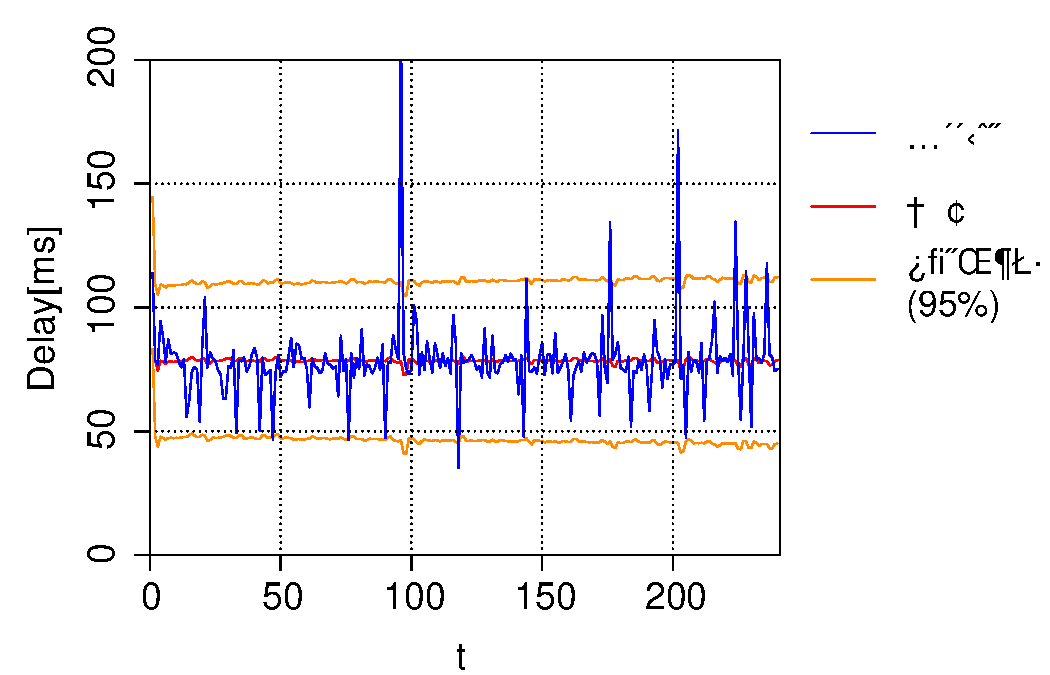
\includegraphics[width=0.5\hsize]{0302_07-plot.pdf}
}~
\subfigure[3/9(月)7:00-8:00]{
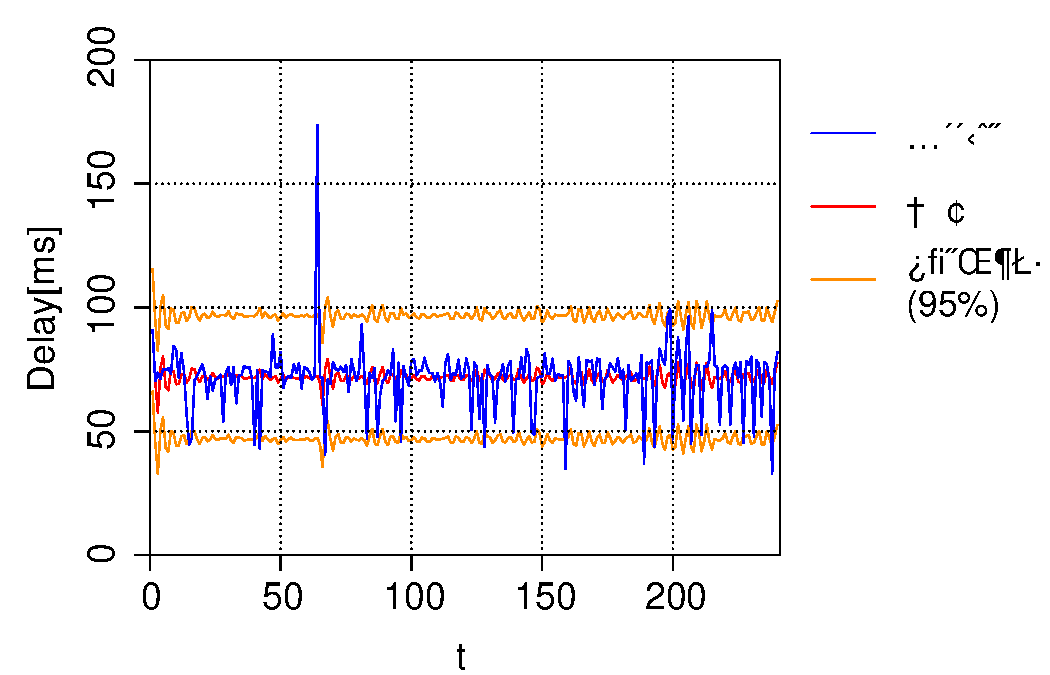
\includegraphics[width=0.5\hsize]{0309_07-plot.pdf}
}
\caption{月曜日の 7:00-8:00 計測の実測値に対する次数 (2,2,1,1) の ARMA-GARCH モデルによる回帰}
\label{norm-reg}
\end{center}
\end{figure}

\begin{table}[tb]
\centering
\caption{図 \ref{norm-reg} に対するモデルのパラメータ}
\label{norm-param}
\begin{tabular}{|c|c|c|}
\hline
&(a) 3/2(月)7:00-8:00&(b) 3/9(月)7:00-8:00\\
\hline
$a_1$&-0.06019205&-0.19235040\\
\hline
$a_2$&-0.11082113&-0.76329719\\
\hline
$b_1$&0.01858739&0.17460199\\
\hline
$b_2$&0.06935663&0.65314854\\
\hline
$c$&91.83487587&140.40728113\\
\hline
$\omega$&0.20250175&8.66125582\\
\hline
$\alpha_1$&0.00000001&0.00000001\\
\hline
$\beta_1$&0.99999999&0.94672654\\
\hline
\end{tabular}
\end{table}

図 \ref{norm-reg} の (a) と (b) の実測値はともに,約 80ms をベースラインとして 40ms から 100ms までの間を激しく変動しており,単発的により大きな値をとっていた.
このように,実測値のベースラインの値や変動範囲には共通性が見られるため,例えば月曜日の 7:00-8:00 に計測したデータにおけるこれらの値が共通の値と大きく異なっていた場合には何らかの異常が発生しているとみなすことができると考える.
一方で, (a) のスパイク発生頻度は (b) よりも多い点や,(b) の最低遅延時間 40ms 程度をとる頻度は (a) よりも多い点は異なっていた.
このように,同じ曜日の同一時間帯に計測したデータであっても,変動の仕方に多少の違いがあるため,実用的な障害検知手法には柔軟性が求められる.
また,(a) と (b) の回帰線はともに,実測値のスパイクや変動にかかわらず概ねベースラインの 80ms 程度に位置していた.
つまり,ARMA-GARCH モデルによる回帰は,スパイクの発生予測は困難であるものの応答遅延のベースラインの変動を捉えることができていると考える.
(a) と (b) の回帰線を細かく見比べてみると,(b) のものは (a) と比べてわずかに変動が激しいように思われる.
したがって,(b) の計測時は (a) の計測時よりも実測値に変動が生じやすい状況であったのではないかと推測される.
また,表 \ref{norm-param} において,各パラメータは (a) と (b) との間で符号やスケールは共通しているが,(b) のパラメータの方が (a) よりも絶対値が僅かに大きい傾向があった.
$a_i$ や $b_i$ の絶対値が大きいほど回帰線の変動が激しくなるため,この違いが図 \ref{norm-reg} の (a) と (b) の回帰線の変動の違いに関係していると思われる.

次に図 \ref{diff-reg} に同区間の変動値に対する回帰結果を示し,表 \ref{diff-param} にそのモデルのパラメータを示す.

\begin{figure}[tb]
\begin{center}
\subfigure[3/2(月)7:00-8:00]{
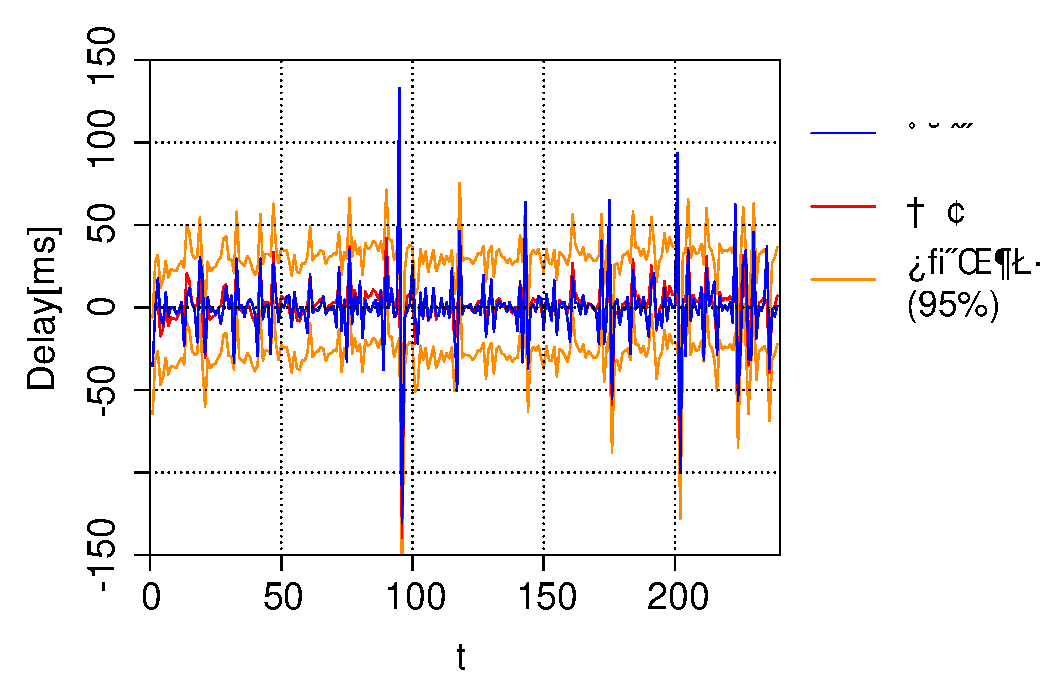
\includegraphics[width=0.5\hsize]{0302_07-plot-diff.pdf}
}~
\subfigure[3/9(月)7:00-8:00]{
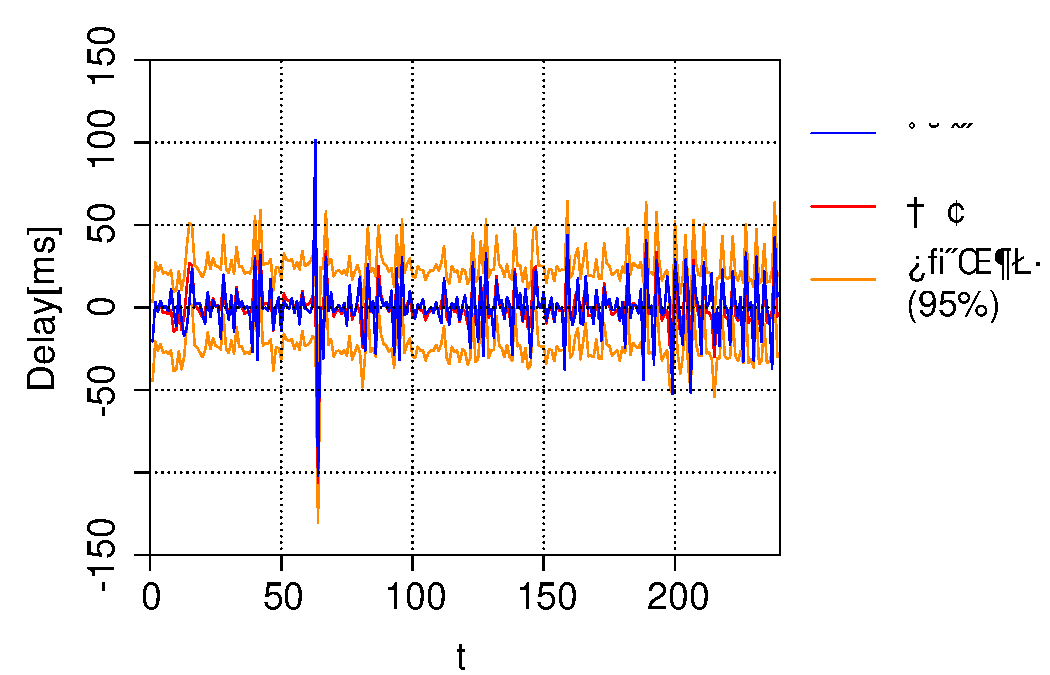
\includegraphics[width=0.5\hsize]{0309_07-plot-diff.pdf}
}
\caption{月曜日の 7:00-8:00 計測の変動値に対する次数 (2,2,1,1) の ARMA-GARCH モデルによる回帰}
\label{diff-reg}
\end{center}
\end{figure}

\begin{table}[tb]
\centering
\caption{図 \ref{diff-reg} に対するモデルのパラメータ}
\label{diff-param}
\begin{tabular}{|c|c|c|}
\hline
&(a) 3/2(月)7:00-8:00&(b) 3/9(月)7:00-8:00\\
\hline
$a_1$&-0.22605053&-0.67683663\\
\hline
$a_2$&-0.06377989&-0.01662159\\
\hline
$b_1$&-0.90702979&-0.42991003\\
\hline
$b_2$&-0.17145273&-0.67824234\\
\hline
$c$&-0.07518171&-0.08615516\\
\hline
$\omega$&166.42677036&8.33052597\\
\hline
$\alpha_1$&0.00000001&0.00000001\\
\hline
$\beta_1$&0.25766368&0.94593359\\
\hline
\end{tabular}
\end{table}

図 \ref{diff-reg} の (a) と (b) の変動値はともに 0 を中心として -50ms から 50ms のまでの範囲を激しく上下していた.
つまり,応答遅延は短期的に激しく変動するものの,長期的に見た変動は 0 に近しくなるようだ.
一方で,図 \ref{diff-reg} では,大きな変動値の次にその符号を逆にした程度の小さな変動値を取る点は図 \ref{norm-reg} と異なる.
この変動部分は実測値におけるスパイクに対応していると思われる.
したがって,大きな変動値に付随して小さな変動値が発生しない場合は,大きな応答遅延が単発的ではなく連続で発生する異常が生じたと考えられる.
また,図 \ref{diff-reg} の (a) と(b) の回帰線はともに変動値のベースライン付近に概ね位置しつつ,スパイクの立下り時にはそれを予測し負に大きな値を取っていた.
この点において,変動値を用いた回帰においては,実測値におけるスパイクの単発性を表現できていると考えられる.
また,表 \ref{diff-param} において,ほとんどのパラメータは表 \ref{norm-param}と同様に, (a) と (b) との間で符号やスケールは共通していたが,(a) の $\omega$ の値は (b) よりもはるかに大きな値となっていた.
これは,(a) の変動値データには (b) よりもスパイクによる上下に大きな変動が多く含まれることが影響しているのではないかと考えられる.

以上の結果より,時系列モデリングによる異常検知においては,前もって定めたモデルパラメータのもとで回帰予測を行っておき,そのベースラインの予測値と実際の計測値を対比させ,結果が大きく外れ続けた場合に異常を検知するものや,工場内部の無線端末上で一定時間幅ごとにリアルタイムに回帰分析を行い,その結果定まるモデルパラメータをベースラインの変化の時間依存性を定量化したものとみなし,前の時間幅におけるモデルパラメータと大きく異なった場合に異常を検知するものなどが考えられる.

\begin{center}
Raspberry Pi の動作不良のため未使用の計測データ\\
3/6(金)17:00-18:00,3/7(土)17:00-18:00\\
3/12(木)12:00-13:00,3/12(木)17:00-18:00\\
3/13(金)17:00-18:00,3/14(土)17:00-18:00\\
3/15(日)17:00-18:00,3/16(月)17:00-18:00\\
3/17(火)20:00-21:00,3/20(金)17:00-18:00\\
3/22(日)17:00-18:00,3/23(月)12:00-13:00\\
3/23(月)20:00-21:00,3/24(火)17:00-18:00\\
3/24(火)20:00-21:00,3/25(水)20:00-21:00\\
3/26(木)20:00-21:00,3/27(金)20:00-21:00\\
\end{center}
\section{クラスタリングによる分類}
 ARMA-GARCH モデルを実測値データもしくは変動値データに対して適用した結果定まるパラメータ $\vector{W}$ をもとにクラスタリングを行い,曜日や時間帯ごとの ping 応答遅延特性を分析する.
$\vector{W}$ は,実測値データと変動値データともに式 (\ref{W}) で与えられる. 
\begin{equation}
\vector{W} = [a_1, a_2, b_1, b_2, c, \omega, \alpha_1, \beta_1]
\label{W}
\end{equation}

$\vector{W}$ の各パラメータの分布帯は異なっているため,パラメータごとに値の解釈は異なる.
そこで,値の解釈を統一するために各パラメータごとの分布がすべて平均 0 の分散が 1 となるように標準化を行った.
標準化後のパラメータ $\vector{W'} = [w'_x1, w'_x2,...,w'_{xn}]$ は,パラメータを $\vector{W} = [w_1,w_2,...,w_n]$,$w_i$ の標準偏差を $s_i$,平均を $M_i$ ,データ $\vector{x}$ に対するパラメータ $[w_{x1},w_{x2},...,w_{x8}]$ として,式 (\ref{standard}) で定められる.
\begin{equation}
w'_{xi} = \frac{w_{xi} - M_i}{s_i}
\label{standard}
\end{equation}

また,クラスタリングにおける次元数が多過ぎると各要素を必要以上に細分化して捉えてしまい,本来同一の傾向がある要素が異なるクラスタに収容されてしまうことが起こり得る.
そのため,クラスタリングに用いるパラメータは各計測データを必要最低限の数で表現したものが望ましい.
本報告では,$\vector{W'}$ に対し主成分分析\cite{jolliffe2016principal}を行い次元を圧縮した.
主成分分析とは,相関のあるパラメータ同士を一つにまとめ,より少ない次元数のもと要素を表現する手法である.
実測値および変動値におけるパラメータ $\vector{W'}$ のそれぞれに対し主成分分析を行った結果の累積寄与率を表 \ref{comp-load} に示す.

\begin{table}[tb]
\begin{center}
\caption{累積寄与率}
\label{comp-load}
\subfigure[実測値に対して]{
\begin{tabular}{|l|l|l|l|}
\hline
第一主成分&第二主成分&第三主成分&第四主成分\\
\hline
0.449& 0.681& 0.863& 0.968\\
\hline
\end{tabular}
}\\
\subfigure[変動値に対して]{
\begin{tabular}{|l|l|l|l|}
\hline
第一主成分&第二主成分&第三主成分&第四主成分\\
\hline
0.367& 0.653& 0.794& 0.905\\
\hline
\end{tabular}
}
\end{center}
\end{table}

主成分を用いた分析を行うには,第一主成分から第何主成分までを用いるかを決める必要があるが,本報告では一般的な判断基準である累積寄与率が 80\% 前後を境とした.
表 \ref{comp-load} より,実測値データと変動値データともに第三主成分までをもとにクラスタリングを行うこととする.
また,実測値および変動値における第三主成分までの主成分負荷量を表 \ref{comp-param} に示す.
表 \ref{comp-param} において,実測値と変動値の第一主成分はともに $a_1$,$b_1$,$b_2$ が大きく寄与していた.
このことから,実測値データおよび変動値データの変動の仕方は,一時点前の実測値および変動値と二時点前までの推定誤差との相関が大きく関係していることがわかる.
一方で,実測値データの第一主成分にはさらに $c,a_2$ も大きく寄与している点で変動値データとの違いが見られた.
\begin{table}[tb]
\begin{center}
\caption{主成分負荷量}
\label{comp-param}
\subfigure[実測値に対して]{
\begin{tabular}{|l|l|l|l|}
\hline
&第一&第二&第三\\
&主成分&主成分&主成分\\
\hline
$c$&0.515&0.133& \\
$a_1$&-0.418&&-0.490\\
$a_2$&-0.404&-0.166&0.492\\
$b_1$&0.424&&0.475\\
$b_2$&0.391&0.157&-0.516\\
$\omega$&-0.119&0.569&0.101\\
$\alpha_1$&-0.142&0.432&\\
$\beta_1$&0.175&-0.643&-0.111\\
\hline
\end{tabular}
}~
\subfigure[変動値に対して]{
\begin{tabular}{|l|l|l|l|}
\hline
&第一&第二&第三\\
&主成分&主成分&主成分\\
\hline
$c$&&&0.721\\
$a_1$&0.571&&\\
$a_2$&&-0.190&-0.067\\
$b_1$&-0.571&&\\
$b_2$&0.574&&\\
$\omega$&&0.553&-0.127\\
$\alpha_1$&&0.499&\\
$\beta_1$&&-0.629&\\
\hline
\end{tabular}
}
\end{center}
\end{table}

クラスタリング手法には様々なものが存在するが,本報告では階層クラスタリングを用いる\cite{fraley1998many}.
階層クラスタリングは,クラスタリング対象の各要素間の近似度(距離)に基づき,最も近い要素同士を集めてクラスタを形成する手法である.
また,クラスタ数を指定した数と一致させる場合,クラスタ間距離に基づき最も近いものの間でクラスタ融合が起こる.
本研究では,距離関数にユークリッド距離を用いる.
要素 $\vector{x} = [w_{x1},w_{x2},...,w_{xn}]$ と $\vector{y} = [w_{y1},w_{y2},...,w_{yn}]$ との間のユークリッド距離関数 $dist(\vector{x},\vector{y})$ は式 \ref{euclidean} で定められる.
\begin{equation}
dist(\vector{x},\vector{y}) = \sqrt{\sum^n_{i=1}( w_{xi} - w_{yi} )^2}
\label{euclidean}
\end{equation}

また,クラスタ融合手法としてウォード法\cite{murtagh2014ward}を用いる.
ウォード法とは,融合後のクラスタ内分散から融合前の二つのクラスタ内分散の差を最小とするという基準でクラスタを融合する手法である.
クラスタリングにおける要素集合 $C$ の代表点には式 (\ref{medoid}) で表されるメドイド\cite{mouratidis2005medoid}を用いる.
\begin{equation}
\argmin_{\vector{x} \in C} \sum_{\vector{y} \in C - \{\vector{x}\}} dist(\vector{x},\vector{y})
\label{medoid}
\end{equation}

クラスタリングを行うにあたり,あらかじめクラスタ数を設定しておく必要がある.
本報告では,クラスタリング指標の一つ PseudoF\cite{liu2010understanding} に我々の研究グループが改良を加えた指標 PseudoF with Min \cite{kanajiri}を用いて定量的に最適なクラスタ数を求める.
PseudoF with Min は式 (\ref{PseudoFwithMin}) で与えられる.
\begin{equation}
\frac{\sum^k_{i=1} n_{i}\hspace{0.1cm} \min \{ dist(\vector{m_{i}},\vector{m_j})^2,j \neq i \}}{1 + \sum^k_{i=1} \sum_{\vector{x} \in C_i - \{\vector{m_i}\}} dist(\vector{x},\vector{m_{i}})^2}
\label{PseudoFwithMin}
\end{equation}
$k$ はクラスタ数とし,各クラスタ集合を $C_1,C_2,...,C_k$ と表す.
$n_i$ はクラスタ $C_i$ に属する要素数であり,$N$ は全要素数である.
また,$\vector{m_i}$ はクラスタ $C_i$ のメドイドであり,$\vector{m}$ は全要素に対するメドイドである.
PseudoF with Min はクラスタ間のばらつき具合を表す分子部分と,クラスタ内のばらつき具合を表す分母部分から構成されており,PseudoF with Min の値が大きいほどクラスタ間は疎でクラスタ内は密であることを意味する.
一般的にクラスタ間は疎でクラスタ内は蜜となったクラスタリング結果が好ましいとされているため,PseudoF with Min の値を大きくするようなクラスタ数を設定する.
実測値および変動値のそれぞれにおいて,クラスタ数に対する PseudoF with Min の値は図 \ref{PseudoFwithMinPlot} となった.
図 \ref{PseudoFwithMinPlot}(a) より,実測値における PseudoF with Min の値はクラスタ数 8 で最大となっており,図 \ref{PseudoFwithMinPlot}(b) より,変動値におけるものはクラスタ数 4 で最大となることが読み取れる.
したがって,実測値の主成分を用いたクラスタリングにおけるクラスタ数は 8,変動値の主成分を用いたクラスタリングにおけるクラスタ数は 4 とする.

\begin{figure}[tb]
\begin{center}
\subfigure[実測値に対して]{
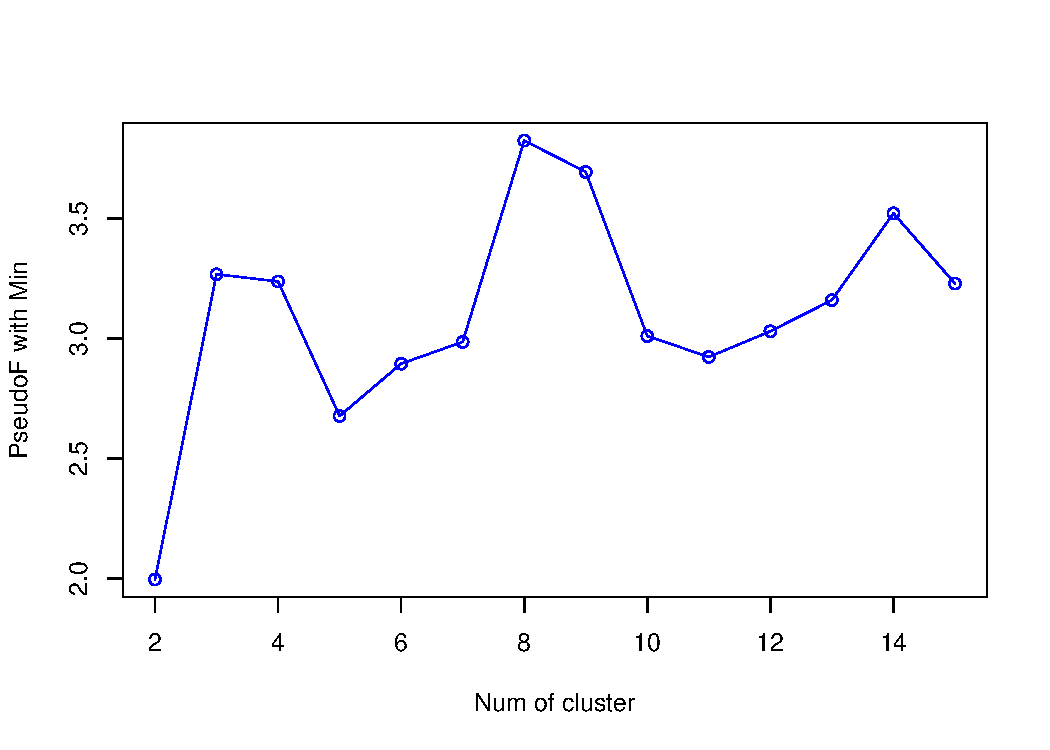
\includegraphics[width=0.5\hsize]{norm_comp-PseudoFwithMin.pdf}
}~
\subfigure[変動値に対して]{
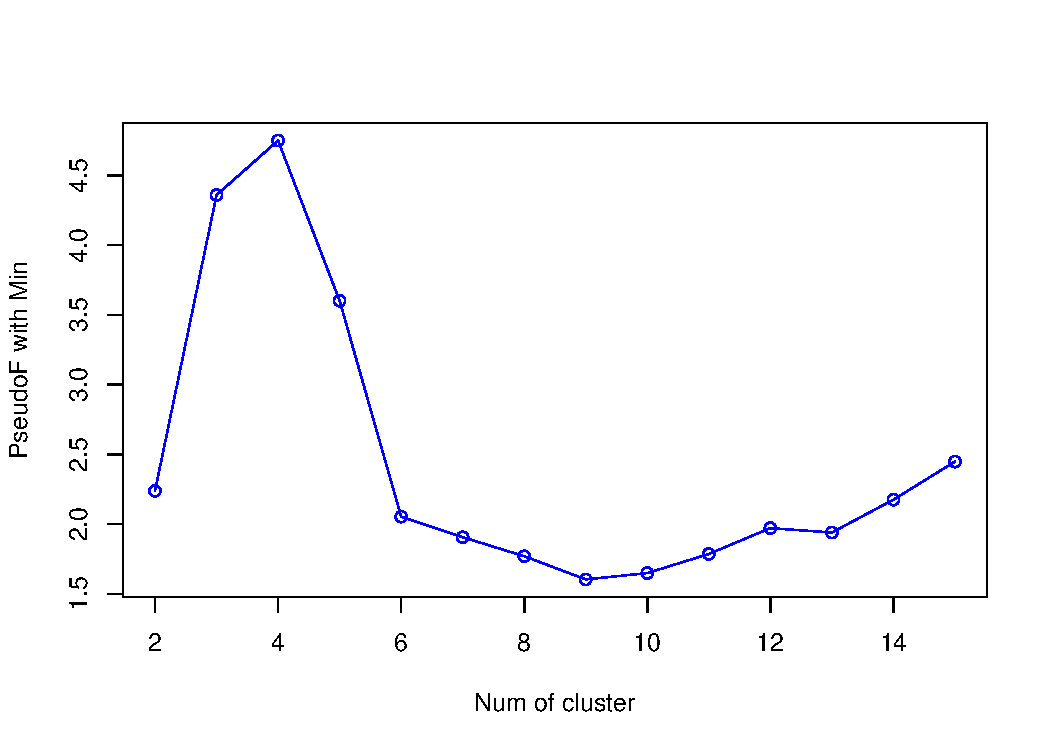
\includegraphics[width=0.5\hsize]{diff_comp-PseudoFwithMin.pdf}
}
\caption{各クラスタ数における PseudoF with Min}
\label{PseudoFwithMinPlot}
\end{center}
\end{figure}

このもとでクラスタリングを行った結果を図 \ref{norm} と図 \ref{diff} に示す.
(a)横軸をクラスタ番号とし計測した時間帯ごとに色分けした積み上げ棒グラフ,(b) 横軸をクラスタ番号とし計測した曜日ごとに色分けした積み上げ棒グラフ,(c)横軸を計測した曜日と時間帯とし属するクラスタ番号ごとに色分けした積み上げ棒グラフである.
縦軸は割合とし,各棒の上部にその要素数を示している.

\begin{figure}[tb]
\begin{center}
\subfigure[時間帯ごとに属するクラスタ]{
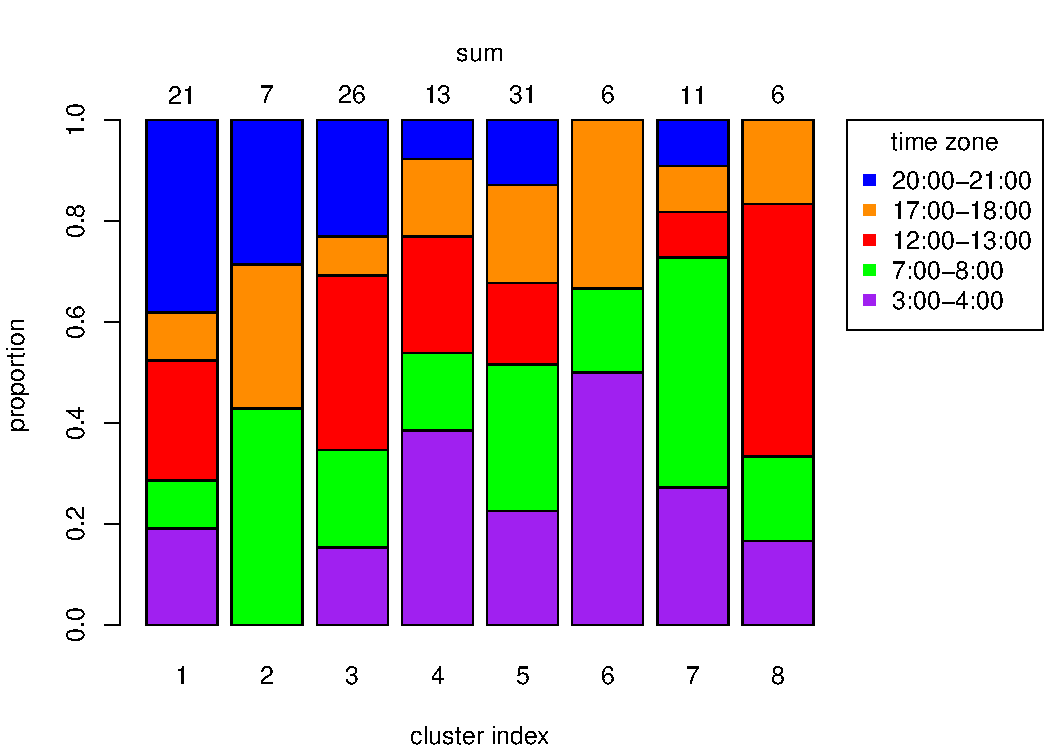
\includegraphics[width=0.5\hsize]{norm_comp-eucl-ward-8-timezone.pdf}
}~
\subfigure[曜日ごとに属するクラスタ]{
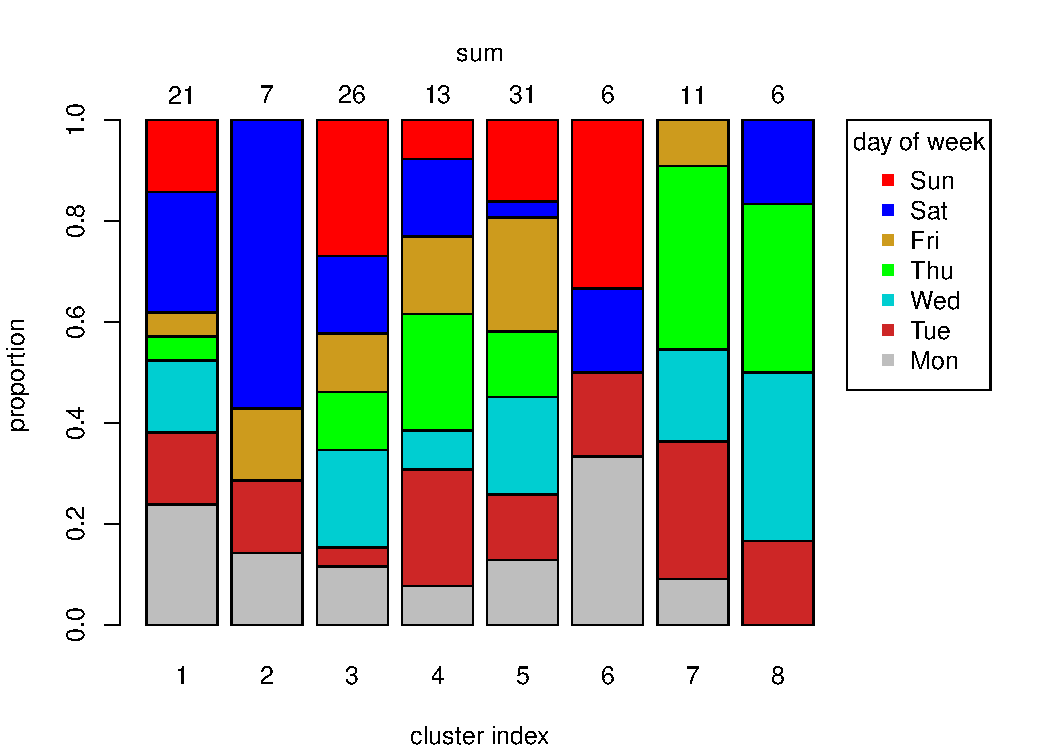
\includegraphics[width=0.5\hsize]{norm_comp-eucl-ward-8-day.pdf}
}\\
\subfigure[各時間帯と曜日が属するクラスタ]{
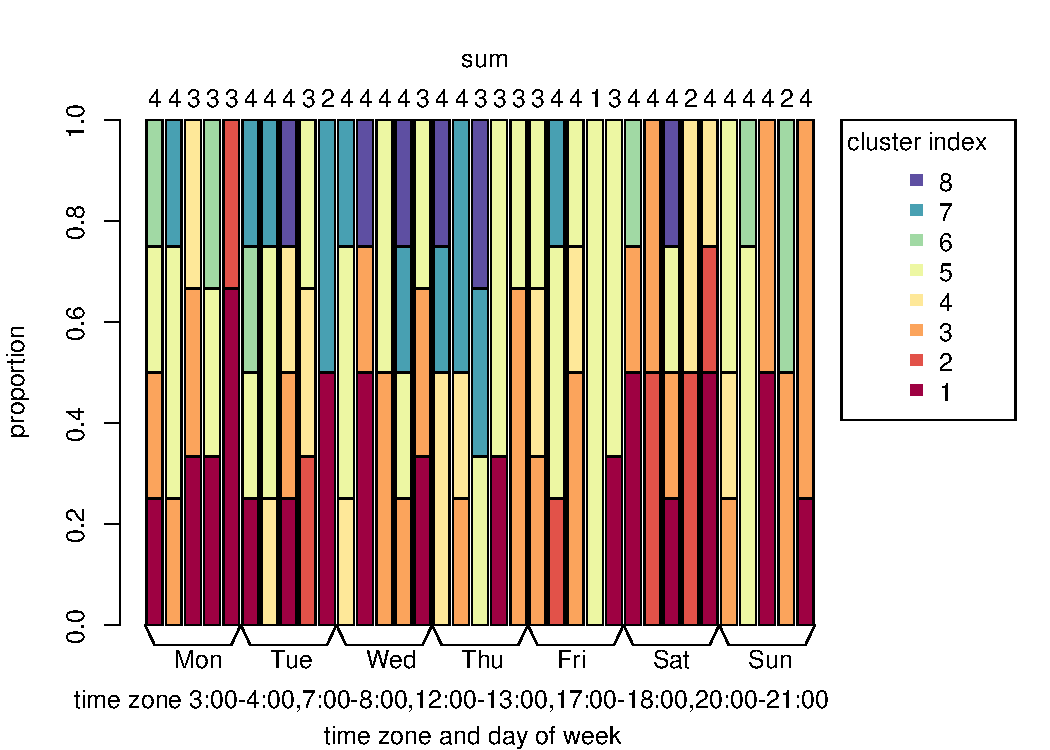
\includegraphics[width=0.5\hsize]{norm_comp-eucl-ward-8-timezone-day.pdf}
}
\caption{実測値の主成分をもとにクラスタ数 8 で行ったクラスタリング結果}
\label{norm}
\end{center}
\end{figure}

\begin{figure}[tb]
\begin{center}
\subfigure[時間帯ごとに属するクラスタ]{
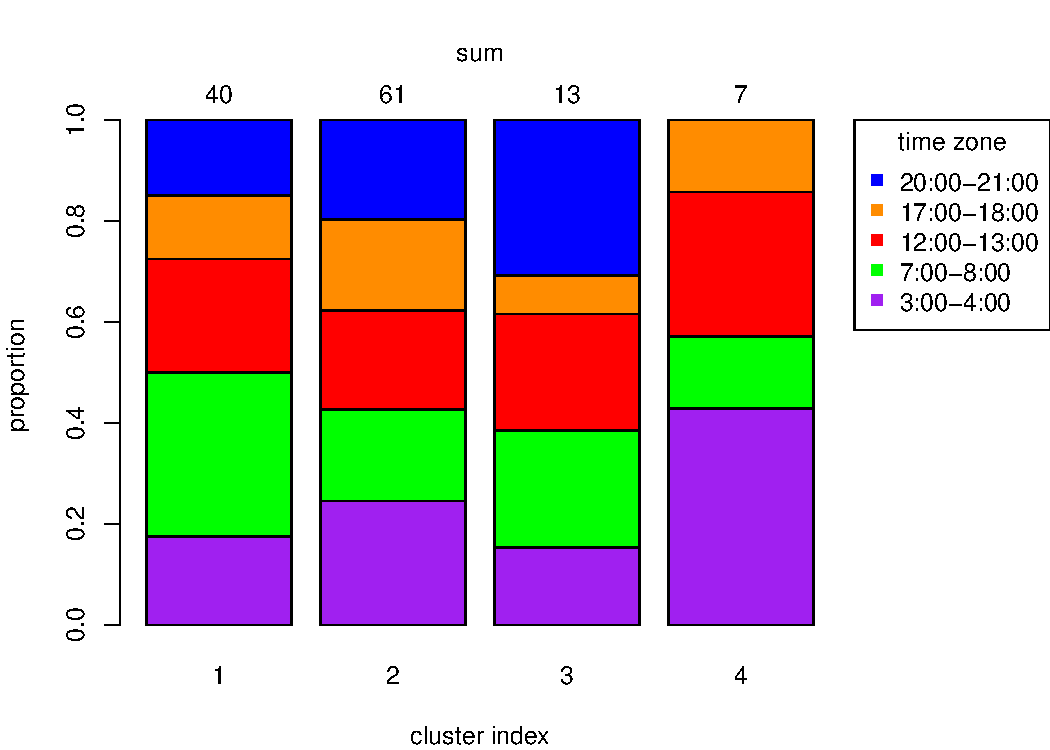
\includegraphics[width=0.5\hsize]{diff_comp-eucl-ward-4-timezone.pdf}
}~
\subfigure[曜日ごとに属するクラスタ]{
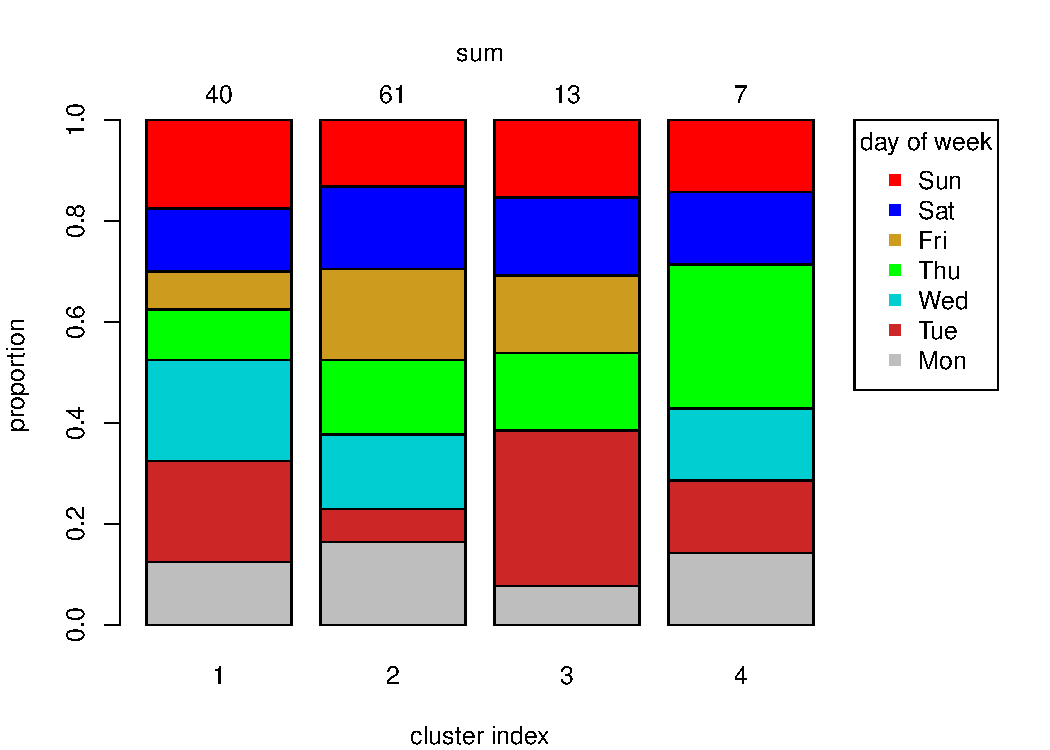
\includegraphics[width=0.5\hsize]{diff_comp-eucl-ward-4-day.pdf}
}\\
\subfigure[各時間帯と曜日が属するクラスタ]{
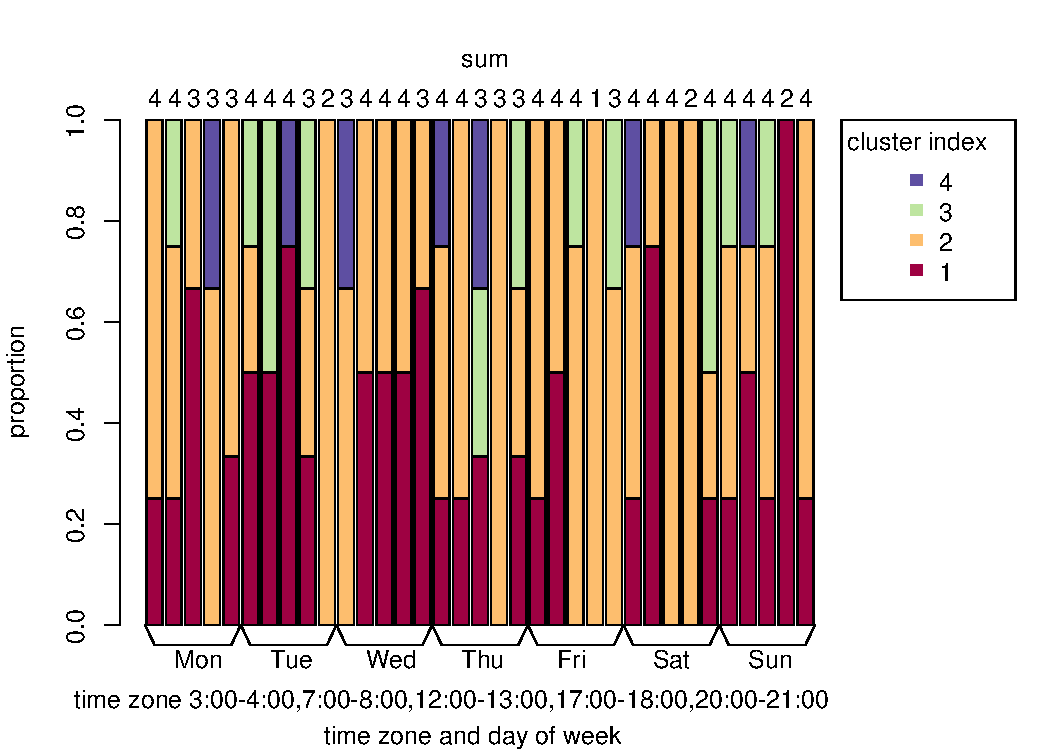
\includegraphics[width=0.5\hsize]{diff_comp-eucl-ward-4-timezone-day.pdf}
}
\caption{変動値の主成分をもとにクラスタ数 4 で行ったクラスタリング結果}
\label{diff}
\end{center}
\end{figure}

図 \ref{norm}(a) のクラスタ番号 1 には 20:00 - 21:00 に計測したデータが多く属しており,図 \ref{norm}(c) より全ての曜日の 20:00 - 21:00 の計測データのうち少なくとも一つはクラスタ番号 1 に属していたため,このクラスタには 20:00 - 21:00 の計測データが属しやすいといえそうだ.
ただ,他のクラスタ番号において全曜日の同一時間帯に計測されたデータが属するクラスタは見受けられなかった.
図 \ref{norm}(a) のクラスタ番号 1 と 3 は,利用者が多いと考えられる 12:00 - 13:00,17:00-18:00,20:00-21:00 の計測データの割合が多い.
さらに,図 \ref{norm}(b) のクラスタ番号 1 と 3 は,利用者が多いと考えられる土曜日と日曜日の割合が多い.
これは図 \ref{norm}(c) からも読み取れる.
したがって,クラスタ番号 1 と 3 には,利用者が多い状況で計測されたデータが属しやすい傾向があるのではないかと考えられる.
逆に図 \ref{norm}(a) のクラスタ番号 7 は,利用者が少ないと考えられる 3:00 - 4:00,7:00 - 8:00 の計測データが多く,図 \ref{norm}(b) のクラスタ番号 7 には利用者が多いと考えられる土曜日と日曜日に計測されたデータは属していなかった.
したがって,クラスタ番号 7 には,利用者が多くない状況で計測されたデータが属しやすい傾向があるのではないかと考えられる.
要素数が少ないクラスタであるクラスタ番号 2 と 6 と 8 のそれぞれにおいて,同一時間帯や同一曜日,または同一の時間帯と曜日のデータが,この他のデータ集合から外れたクラスタに属する傾向があるかを調べたが,この結果からはそのような傾向は見受けられなかった.
以上より,実測値の主成分によるクラスタリングを用いた異常検知方法としては,時間帯や曜日ごとにモデルパラメータのテンプレートをその傾向を捉えたクラスタの代表点から用意し,その下で回帰予測を行い得られる応答遅延のベースラインの予測値から実測値が大きく外れ続けた場合に異常を検知する手法や,現場の無線端末上でリアルタイムに逐次クラスタリングを行い,その計測データが収容されるクラスタが時間帯や曜日の傾向を捉えたクラスタから外れ続けた場合に異常を検知する手法などが考えられる.

図 \ref{diff} の変動値の主成分によるクラスタリングでは,多くのデータが図 \ref{diff}(a) のクラスタ番号 1 か 2 に属していた.
図 \ref{diff}(c) からはどの曜日のどの時間帯においてもまんべんなくクラスタ番号 1 か 2 に属していることが見て取れる.
またこれらのクラスタから外れた要素数の少ないクラスタのクラスタ番号 3 か 4 に属するデータには,計測時間帯や曜日に共通性は見て取れない.
したがって,変動値はおおよそクラスタ番号 1 か 2 で代表され,そこから外れる場合もあるがそこに共通性はなさそうだ.
よって,変動値の主成分によるクラスタリングを用いた異常検知方法としては,現場の無線機器で一定の時間幅の取得データをもとにクラスタリングを行い,要素数の多いクラスタから外れ続けた場合に異常を検知する手法などが考えられる.

\section{まとめと今後の課題}
本報告では,応答遅延の実測値および変動値のベースラインの時間経過に伴う変動の仕方を ARMA-GARCH モデルのモデルパラメータから捉えることが可能であることを示した.
さらに,標準化されたモデルパラメータの第三主成分までを用いてクラスタリングを行うことで,その時間帯や曜日に応じたある傾向を捉えられることが可能であること示した.
これにより,ARMA-GARCH モデルを用いて応答遅延の実測値および変動値のベースラインの変動の仕方を求め,通常の傾向と対比して行う異常検知手法が可能と考える.
障害検知手法としては,例えば,前もって行ったクラスタリング結果において形成された曜日や時間帯ごとの傾向を持つクラスタの代表点を,その曜日や時間帯における ARMA-GARCH モデルのパラメータのテンプレートとし,それを用いて行った応答遅延の予測値から実測値が大きく外れ続けた場合に異常を検知する手法が考えられる.
または,現場の無線機器で逐次クラスタリングを行った結果が,その計測時における曜日や時間帯の傾向を持つクラスタに属さなかった場合に異常を検知する手法も考えられる.

今後の課題として,曜日や時間帯ごとの傾向はありそうだがそれは顕著なものではなかったため,クラスタリング結果に基づいた異常検知手法だけでは誤検知や検知漏れが発生すると考えられる.
そのため,実用するにあたっては,時系列解析ベースで異常検知を行いながら他の手法と組み合わせる必要があると考える.
それには例えば,時系列モデルを用いた回帰分析から大きく外れるものつまりはスパイクの発生頻度や大きさが通常時とは異なる場合に異常を検知する手法などが考えられる.

\bibliography{myrefs}
\bibliographystyle{sieicej}
\end{document}